\section{Introduction}\label{sec:introduction}
%\cleet{Introduction placeholder text}
A major research direction of SDN is programmable, efficient datapaths (\eg, OF1.3~\cite{openflow13}, OF-DPA~\cite{OF-DPA}, P4~\cite{P4}). Only by being programmable can a given SDN datapath support diverse, ever evolving application scenarios. At the same time, it is crucial that datapaths be efficient, to be able to satisfy demanding requirements such as achieving high throughput and being cost effective. In the last few years, multi-table pipelines have emerged as a key structure of SDN datapaths (\eg, Domino~\cite{Domino}, Forwarding Metamorphosis~\cite{bosshart2013forwarding}). 

%A problem of efficient datapaths, however, is that they can be low level to program.

One problem of efficient datapaths, however, is that they must often be programmed at an inefficiently low level. For example, TCAM, which is essential to achieve high-throughput, does not support logical negation. Hence, a second major research direction of SDN is high-level, datapath path-oblivious programming, to provide abstractions to hide low-level datapath programming. To this end, in the last few years multiple high-level SDN programming models have emerged (\eg, Frenetic~\cite{frenetic}, Maple~\cite{maple}).

As both directions progress, a basic problem emerges: whether a given high-level program can be realized on a given low-level datapath. A good understanding of this problem can benefit both the design of high-level SDN programming and the design of datapaths. Given a fixed datapath (\eg, a fixed pipeline architecture such as OF-DPA), the vendor of the datapath can provide guidelines on the high-level programs that can be realized. Given a set of high-level programs to be supported, one could use this understanding to design the most compact datapath supporting these programs. Even for reconfigurable datapaths (\eg, P4), as reconfiguration can be expensive and time consuming, one can use this understanding to guide the design of a more robust datapath. Considering all high-level programs that can be realized onto a given programmable datapath as the capacity of the datapath, we define the basic problem as the {\em SDN datapath programming capacity problem}.

%\begin{figure}[h!]
%    \centering
%    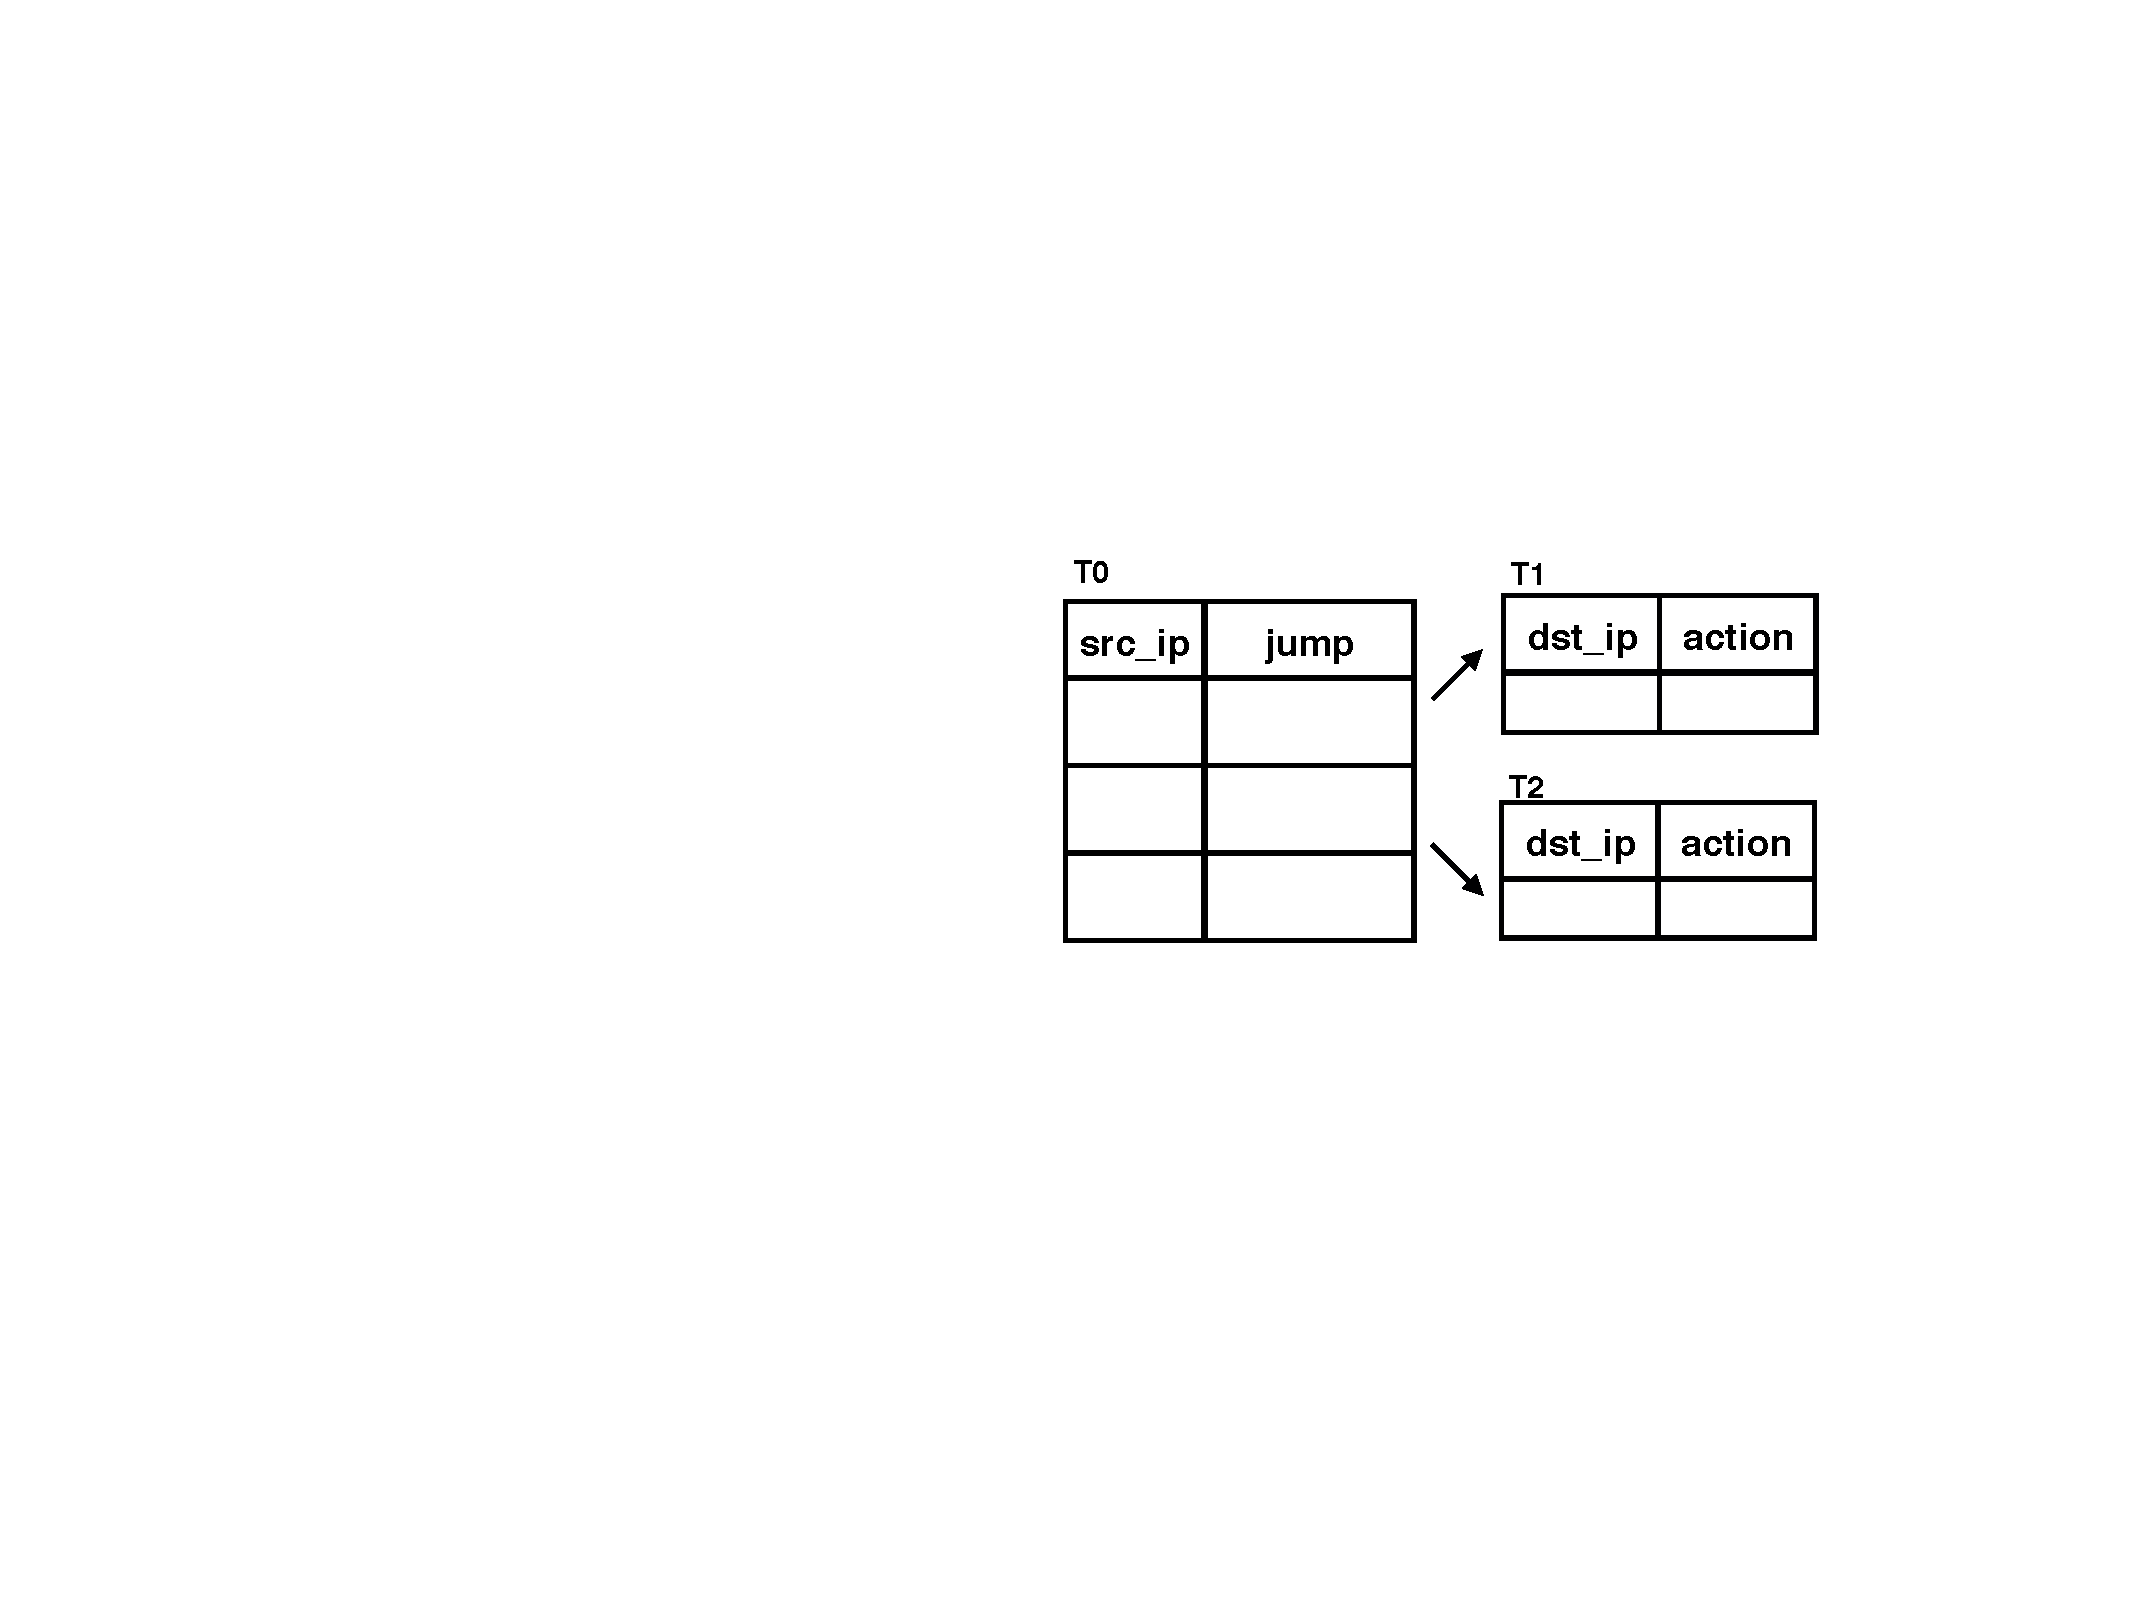
\includegraphics[width=3.25in]{figures/fig1-update.pdf}
%%    \vspace{-0.3in}
%    \caption{Example datapath.}
%    \label{fig:fig1-update}
%\end{figure}

% Solving the datapath programming capacity problem, however, is not trivial. Consider a high-level program \texttt{onPkt} shown in Sec.~\ref{sec:model-and-main-results}. The if statements in the program make the structure complex and the flexibility of table design makes the formalization of program hard. It is not desirable to make much restriction on programmers when they are writing high-level programs. Also, from the other side, consider a pipeline \texttt{swP} shown in Sec.~\ref{sec:model-and-main-results} Though the pipeline \texttt{swP} also defines a set tables, the layout might be different with the program \texttt{onPkt}, which including the pipeline structure and table matching fields. For example, the program \texttt{onPkt} requires a table matching both $dstAddr$ and $dstPort$ which does not exist in the pipeline \texttt{swP}. It is not obvious to see whether the program can be realized on the pipeline. 




%Fig.~\ref{fig:fig1-update}, which shows a simple datapath, named Example-DP, which consists of two-tables forming a pipeline. 
%Consider two simple high-level SDN programs [revise]. An interested reader can try to verify that the first program can be realized by Example-DP, but the second cannot. 
%{\small
%\begin{verbatim}
%// Program: L3-Route
%
%   onPacket(p):
%1.   s = p.srcIP
%2.   d = p.dstIP
%3.   if (s == "10.0.0.1"):
%4.     egress = myPolicyOne(d)
%5.   else
%6.     egress = myPolicyTwo(d)
%8.   return egress
%\end{verbatim}
%}
%
%{\small
%\begin{verbatim}
%// Program: L3-Route-Changed
%...
%4.   if (s == "10.0.0.1"):
%5.     egress = myPolicyOne(d)
%6.   else if (s == "10.0.0.2"):
%7.     egress = my PolicyThree(d)
%...
%\end{verbatim}
%}

%Consider a high-level program \texttt{onPkt} shown in Sec.~\ref{sec:model-and-main-results}. The if statements in the program make the structure complex and the flexibility of table design makes the formalization of program hard. It is not desirable to make much restriction on programmers when they are writing high-level programs. Also, from the other side, consider a pipeline \texttt{swP} shown in Sec.~\ref{sec:model-and-main-results} Though the pipeline \texttt{swP} also defines a set tables, the layout might be different with the program \texttt{onPkt}, which including the pipeline structure and table matching fields. For example, the program \texttt{onPkt} requires a table matching both $dstAddr$ and $dstPort$ which does not exist in the pipeline \texttt{swP}. It is not obvious to see whether the program can be realized on the pipeline. 



Solving the datapath capacity problem, however, is not trivial. 
Consider a simple datapath, named Simple-DP, shown in Fig.~\ref{fig:fig1-update}. It is among the simplest datapaths, consisting of three tables forming a pipeline, where the first table (\texttt{t1}) matches on source IP and may jump to one of the two following tables, which both match on destination IP.
\begin{figure}[h!]
    \centering
    \vspace{-0.1in}
    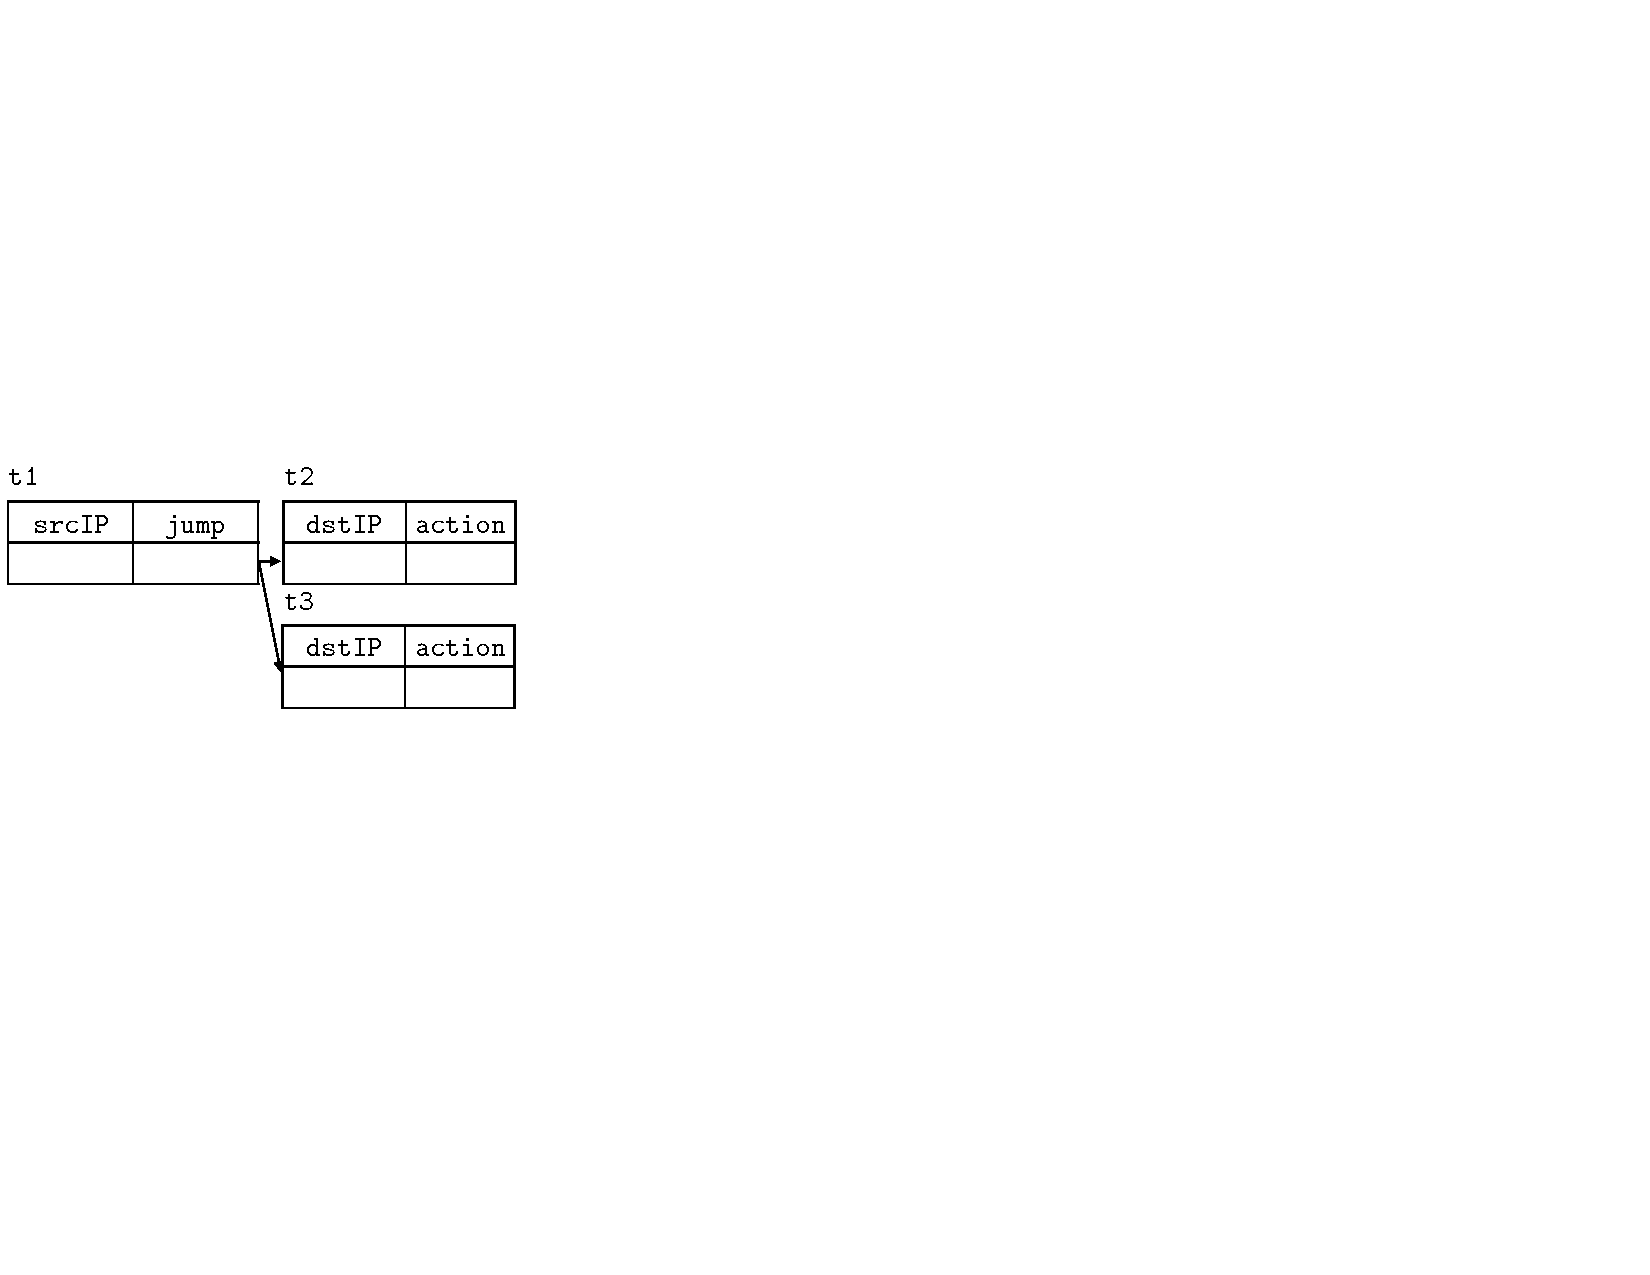
\includegraphics[scale = 0.7]{figures/figure1.pdf}
    \vspace{-0.1in}
    \caption{A simple example datapath: Simple-DP.}
    \vspace{-0.1in}
    \label{fig:fig1-update}
\end{figure}

Consider two simple high-level SDN programs below, both specified in the algorithmic, event-driven programming style to handle packet misses; see Sec. II for more details on the programming model. An interested reader can try to verify that the first program can be realized by Simple-DP, but the second cannot. 
{\small
\begin{verbatim}
//  Routing Function: secureL3Route
L0: secureL3Route(Addr srcIP, Addr dstIP):
L1:   if srcIP == 10.0.0.1:
L2:     return Forward(port=shortestPath(dstIP))
L3:   else:
L4:     return Drop();
\end{verbatim}
}

{\small
\begin{verbatim}
//  Program: twoHostL3Route
L0: def twoHostL3Route(Addr srcIP, Addr dstIP):
L1:   if srcIP == 10.0.0.1:
L2:     return Forward(port=shortestPath(dstIP)) 
L3:   elif srcIP == 10.0.0.2:
L4:     return Forward(port=securePath(dstIP))
L5:   else:
L6:     return Drop();
\end{verbatim}}

Although the preceding datapath and high-level programs are among the simplest, they may already appear to be non-trivial for a reader to analyze. General datapath and high-level programs can be much more complex as multiple services need to be implemented and hence they can pose severe challenges in analysis. The goal of this paper is to develop the first systematic methodology to solve the SDN datapath programming capacity problem. 

The contributions of this paper can be summarized as follows. First, we  propose a unifying characteristic functional space to unify and extract the essence of programs and pipelines, removing complexities such as program structures and pipeline layouts. Second, we define a comparator in this functional space, which can be used to check whether a high-level program can be realized on a given pipeline.

The rest of the paper is organized as follows. We define our model precisely in Sec.~\ref{sec:model-and-main-results}. The main results are given in Sec.~\ref{sec:main-results} and the proofs are shown in Sec.~\ref{sec:proofs}. Sec.~\ref{sec:evaluation} shows our evaluation results. Finally, related work is provided in Sec.~\ref{sec:related-work}.
